% Options for packages loaded elsewhere
\PassOptionsToPackage{unicode}{hyperref}
\PassOptionsToPackage{hyphens}{url}
\PassOptionsToPackage{dvipsnames,svgnames,x11names}{xcolor}
%
\documentclass[
  letterpaper,
  DIV=11,
  numbers=noendperiod]{scrartcl}

\usepackage{amsmath,amssymb}
\usepackage{iftex}
\ifPDFTeX
  \usepackage[T1]{fontenc}
  \usepackage[utf8]{inputenc}
  \usepackage{textcomp} % provide euro and other symbols
\else % if luatex or xetex
  \usepackage{unicode-math}
  \defaultfontfeatures{Scale=MatchLowercase}
  \defaultfontfeatures[\rmfamily]{Ligatures=TeX,Scale=1}
\fi
\usepackage{lmodern}
\ifPDFTeX\else  
    % xetex/luatex font selection
\fi
% Use upquote if available, for straight quotes in verbatim environments
\IfFileExists{upquote.sty}{\usepackage{upquote}}{}
\IfFileExists{microtype.sty}{% use microtype if available
  \usepackage[]{microtype}
  \UseMicrotypeSet[protrusion]{basicmath} % disable protrusion for tt fonts
}{}
\makeatletter
\@ifundefined{KOMAClassName}{% if non-KOMA class
  \IfFileExists{parskip.sty}{%
    \usepackage{parskip}
  }{% else
    \setlength{\parindent}{0pt}
    \setlength{\parskip}{6pt plus 2pt minus 1pt}}
}{% if KOMA class
  \KOMAoptions{parskip=half}}
\makeatother
\usepackage{xcolor}
\setlength{\emergencystretch}{3em} % prevent overfull lines
\setcounter{secnumdepth}{-\maxdimen} % remove section numbering
% Make \paragraph and \subparagraph free-standing
\makeatletter
\ifx\paragraph\undefined\else
  \let\oldparagraph\paragraph
  \renewcommand{\paragraph}{
    \@ifstar
      \xxxParagraphStar
      \xxxParagraphNoStar
  }
  \newcommand{\xxxParagraphStar}[1]{\oldparagraph*{#1}\mbox{}}
  \newcommand{\xxxParagraphNoStar}[1]{\oldparagraph{#1}\mbox{}}
\fi
\ifx\subparagraph\undefined\else
  \let\oldsubparagraph\subparagraph
  \renewcommand{\subparagraph}{
    \@ifstar
      \xxxSubParagraphStar
      \xxxSubParagraphNoStar
  }
  \newcommand{\xxxSubParagraphStar}[1]{\oldsubparagraph*{#1}\mbox{}}
  \newcommand{\xxxSubParagraphNoStar}[1]{\oldsubparagraph{#1}\mbox{}}
\fi
\makeatother


\providecommand{\tightlist}{%
  \setlength{\itemsep}{0pt}\setlength{\parskip}{0pt}}\usepackage{longtable,booktabs,array}
\usepackage{calc} % for calculating minipage widths
% Correct order of tables after \paragraph or \subparagraph
\usepackage{etoolbox}
\makeatletter
\patchcmd\longtable{\par}{\if@noskipsec\mbox{}\fi\par}{}{}
\makeatother
% Allow footnotes in longtable head/foot
\IfFileExists{footnotehyper.sty}{\usepackage{footnotehyper}}{\usepackage{footnote}}
\makesavenoteenv{longtable}
\usepackage{graphicx}
\makeatletter
\def\maxwidth{\ifdim\Gin@nat@width>\linewidth\linewidth\else\Gin@nat@width\fi}
\def\maxheight{\ifdim\Gin@nat@height>\textheight\textheight\else\Gin@nat@height\fi}
\makeatother
% Scale images if necessary, so that they will not overflow the page
% margins by default, and it is still possible to overwrite the defaults
% using explicit options in \includegraphics[width, height, ...]{}
\setkeys{Gin}{width=\maxwidth,height=\maxheight,keepaspectratio}
% Set default figure placement to htbp
\makeatletter
\def\fps@figure{htbp}
\makeatother

\usepackage{booktabs}
\usepackage{longtable}
\usepackage{array}
\usepackage{multirow}
\usepackage{wrapfig}
\usepackage{float}
\usepackage{colortbl}
\usepackage{pdflscape}
\usepackage{tabu}
\usepackage{threeparttable}
\usepackage{threeparttablex}
\usepackage[normalem]{ulem}
\usepackage{makecell}
\usepackage{xcolor}
\KOMAoption{captions}{tableheading}
\makeatletter
\@ifpackageloaded{caption}{}{\usepackage{caption}}
\AtBeginDocument{%
\ifdefined\contentsname
  \renewcommand*\contentsname{Table of contents}
\else
  \newcommand\contentsname{Table of contents}
\fi
\ifdefined\listfigurename
  \renewcommand*\listfigurename{List of Figures}
\else
  \newcommand\listfigurename{List of Figures}
\fi
\ifdefined\listtablename
  \renewcommand*\listtablename{List of Tables}
\else
  \newcommand\listtablename{List of Tables}
\fi
\ifdefined\figurename
  \renewcommand*\figurename{Figure}
\else
  \newcommand\figurename{Figure}
\fi
\ifdefined\tablename
  \renewcommand*\tablename{Table}
\else
  \newcommand\tablename{Table}
\fi
}
\@ifpackageloaded{float}{}{\usepackage{float}}
\floatstyle{ruled}
\@ifundefined{c@chapter}{\newfloat{codelisting}{h}{lop}}{\newfloat{codelisting}{h}{lop}[chapter]}
\floatname{codelisting}{Listing}
\newcommand*\listoflistings{\listof{codelisting}{List of Listings}}
\makeatother
\makeatletter
\makeatother
\makeatletter
\@ifpackageloaded{caption}{}{\usepackage{caption}}
\@ifpackageloaded{subcaption}{}{\usepackage{subcaption}}
\makeatother

\ifLuaTeX
  \usepackage{selnolig}  % disable illegal ligatures
\fi
\usepackage{bookmark}

\IfFileExists{xurl.sty}{\usepackage{xurl}}{} % add URL line breaks if available
\urlstyle{same} % disable monospaced font for URLs
\hypersetup{
  pdftitle={Proportion\_analysis},
  colorlinks=true,
  linkcolor={blue},
  filecolor={Maroon},
  citecolor={Blue},
  urlcolor={Blue},
  pdfcreator={LaTeX via pandoc}}


\title{Proportion\_analysis}
\author{}
\date{}

\begin{document}
\maketitle


\begin{verbatim}
# A tibble: 1 x 3
    age gender referendum
  <int>  <int>      <int>
1    12     18         85
\end{verbatim}

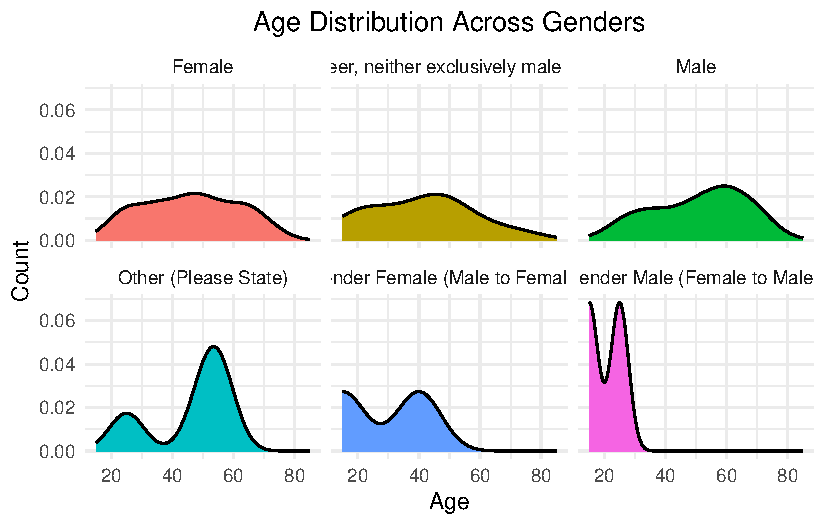
\includegraphics{Proportion_analysis_files/figure-pdf/unnamed-chunk-4-1.pdf}

\section{Complete cases}\label{complete-cases}

\subsubsection{1. The proportion for vote `yes' in the
referendum}\label{the-proportion-for-vote-yes-in-the-referendum}

\begin{verbatim}
[1] 0.6
\end{verbatim}

\subsubsection{2. Logistic regression table for Complete
cases}\label{logistic-regression-table-for-complete-cases}

\begin{longtable}[t]{lrrrr}
\caption{Logistic Regression on Complete Cases}\\
\toprule
term & estimate & std.error & statistic & p.value\\
\midrule
(Intercept) & 1.9911196 & 0.2418370 & 8.2333136 & 0.0000000\\
age & -0.0291008 & 0.0045787 & -6.3557526 & 0.0000000\\
genderGenderqueer, neither exclusively male nor female & 1.3495750 & 1.0764310 & 1.2537496 & 0.2099330\\
genderMale & -0.4127509 & 0.1377062 & -2.9973304 & 0.0027236\\
genderOther (Please State) & 0.2548679 & 1.2291860 & 0.2073469 & 0.8357389\\
\addlinespace
genderTransgender Female (Male to Female: MTF) & 13.3899203 & 608.7668192 & 0.0219952 & 0.9824518\\
genderTransgender Male (Female to Male; FTM) & 13.1592764 & 621.6285024 & 0.0211690 & 0.9831108\\
\bottomrule
\end{longtable}

\section{Imputed cases}\label{imputed-cases}

\subsubsection{1. The proportion of yes
voters}\label{the-proportion-of-yes-voters}

\begin{verbatim}
[1] 0.6
\end{verbatim}

\subsubsection{2. Logistic Regression Table for multiple
imputation}\label{logistic-regression-table-for-multiple-imputation}

\begin{longtable}[t]{lrrrrr}
\caption{Logistic Regression on Imputed Data}\\
\toprule
term & estimate & std.error & statistic & df & p.value\\
\midrule
(Intercept) & 1.9907956 & 0.2615553 & 7.6113766 & 59.81544 & 0.0000000\\
age & -0.0293965 & 0.0048799 & -6.0239461 & 82.77097 & 0.0000000\\
genderGenderqueer, neither exclusively male nor female & 1.3638259 & 1.0773457 & 1.2659131 & 1032.92575 & 0.2058297\\
genderMale & -0.3960150 & 0.1371885 & -2.8866495 & 435.38010 & 0.0040875\\
genderOther (Please State) & 0.5014826 & 1.1705221 & 0.4284264 & 1033.82042 & 0.6684299\\
\addlinespace
genderTransgender Female (Male to Female: MTF) & 13.3989723 & 608.4891979 & 0.0220201 & 1035.89948 & 0.9824362\\
genderTransgender Male (Female to Male; FTM) & 13.1656106 & 621.5790396 & 0.0211809 & 1035.89948 & 0.9831054\\
\bottomrule
\end{longtable}

\section{Conclusion:}\label{conclusion}

Based on the analysis, the proportion of people in the sample who
supported legalisation is 0.59 using complete cases and 0.6 using
imputed data. The logistic regression interpret the results from the
logistic regression output.

\section{Comparison of Regression
Analyses}\label{comparison-of-regression-analyses}

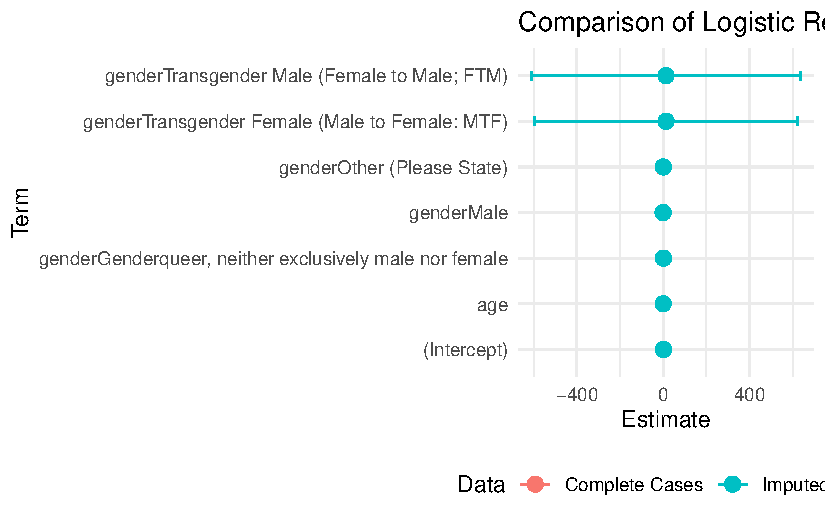
\includegraphics{Proportion_analysis_files/figure-pdf/unnamed-chunk-10-1.pdf}




\end{document}
